\section{Testing eBPF programs}\label{sec:testing}
To verify the correctness of a P4-XDP program, the compiler integrates a full 
end-to-end testing framework. The framework consists of an userspace eBPF 
runtime as well as a kernel testing pipeline, which verifies eBPF/XDP programs 
in a virtual, isolated environment.

\subsection{Why Test in User-Space?}
\begin{itemize}
	\item Test the compiler correctness
	\item Isolate functionality in user-space
	\item C output must be functionally equivalent to P4
	\item Fewer dependencies. Does not require specific versions of Linux 
	kernel llvm Kernel hook or on eBPF verifier
	\item Debugging simplicity (e.g., GDB, printf, valgrind)
\end{itemize}

\subsection{The Simple Test Framework}
\begin{figure}
	\centering
	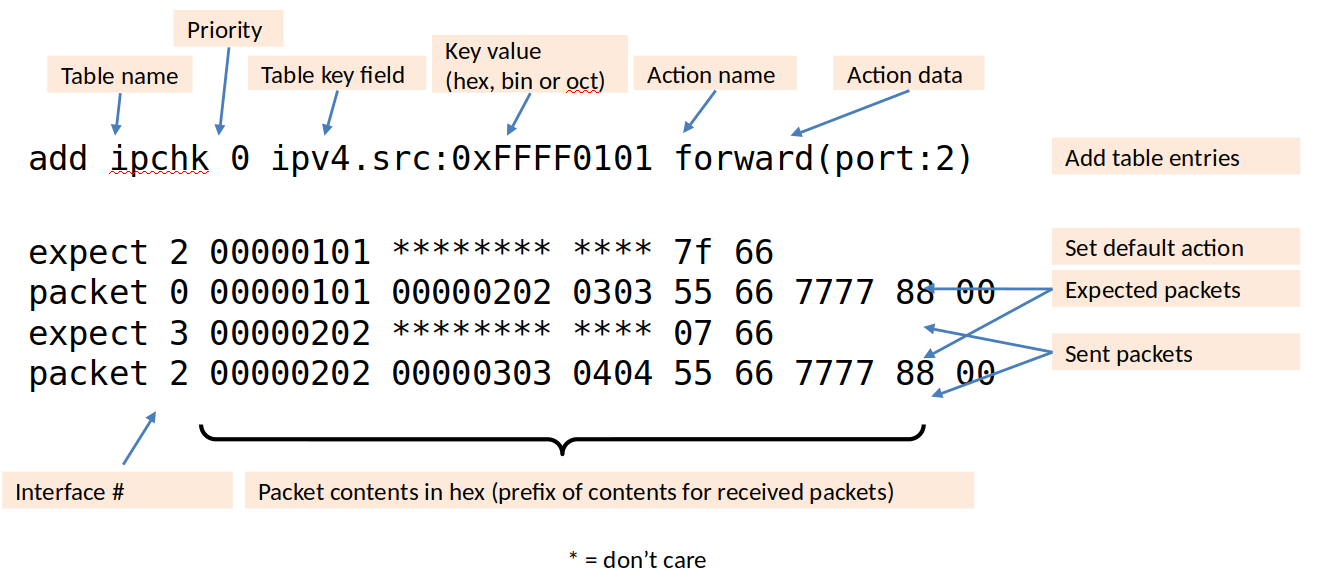
\includegraphics[width=0.7\linewidth]{stf}
	\caption{}
	\label{fig:stf}
\end{figure}
The simple test framework is a data plane verification language, which is used 
by the p4c-ebpf compiler. While its original purpose is to assess switching and 
forwarding behavior, it can also test the functionality of eBPF programs in 
isolation.
In general, an .stf file describes the input as well the expected output 
packets per switch, or in this case virtual bridge, port. In addition, it may 
also define the initial state of the dataplane tables and may contain a list of 
control plane commands which are to be run in sequence....

Compiler comes with a Python parser for STF

\subsection{The Test Runtime}
Describe the userspace runtime.
User-space wrappers around eBPF tables and APIs
\begin{figure}
	\centering
	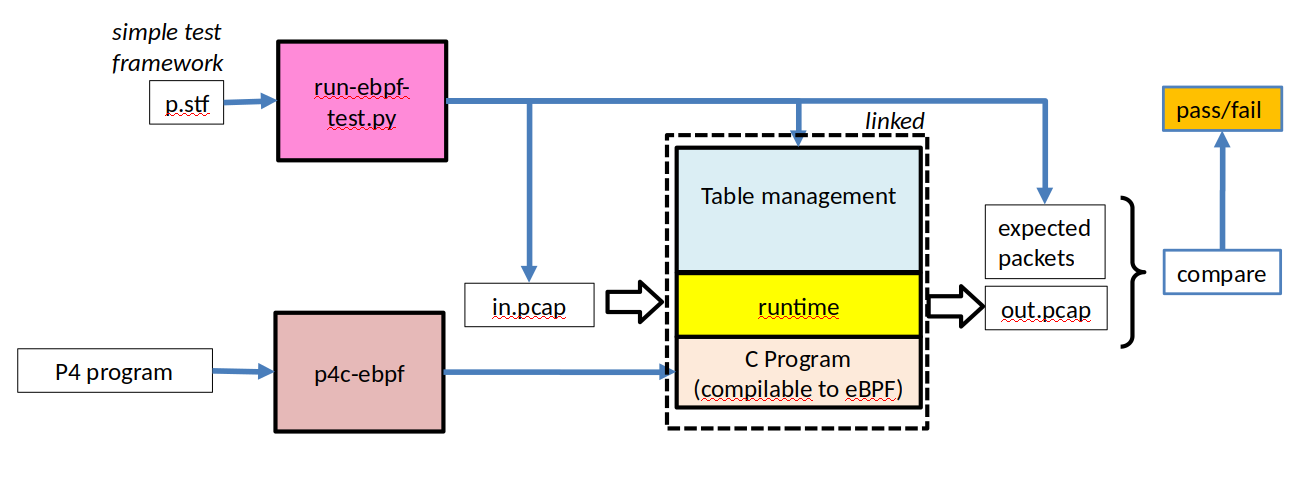
\includegraphics[width=0.7\linewidth]{user_test}
	\caption{}
	\label{fig:user_test}
\end{figure}

\subsection{Testing P4 Programs End-to-End}
Talk about how to use the test framework to verify your eBPF code or p4 file 
end-to-end. Highlight, how the framework can be used to test eBPF and XDP 
programs in general, independent from the P4 pipeline.
\begin{figure}
	\centering
	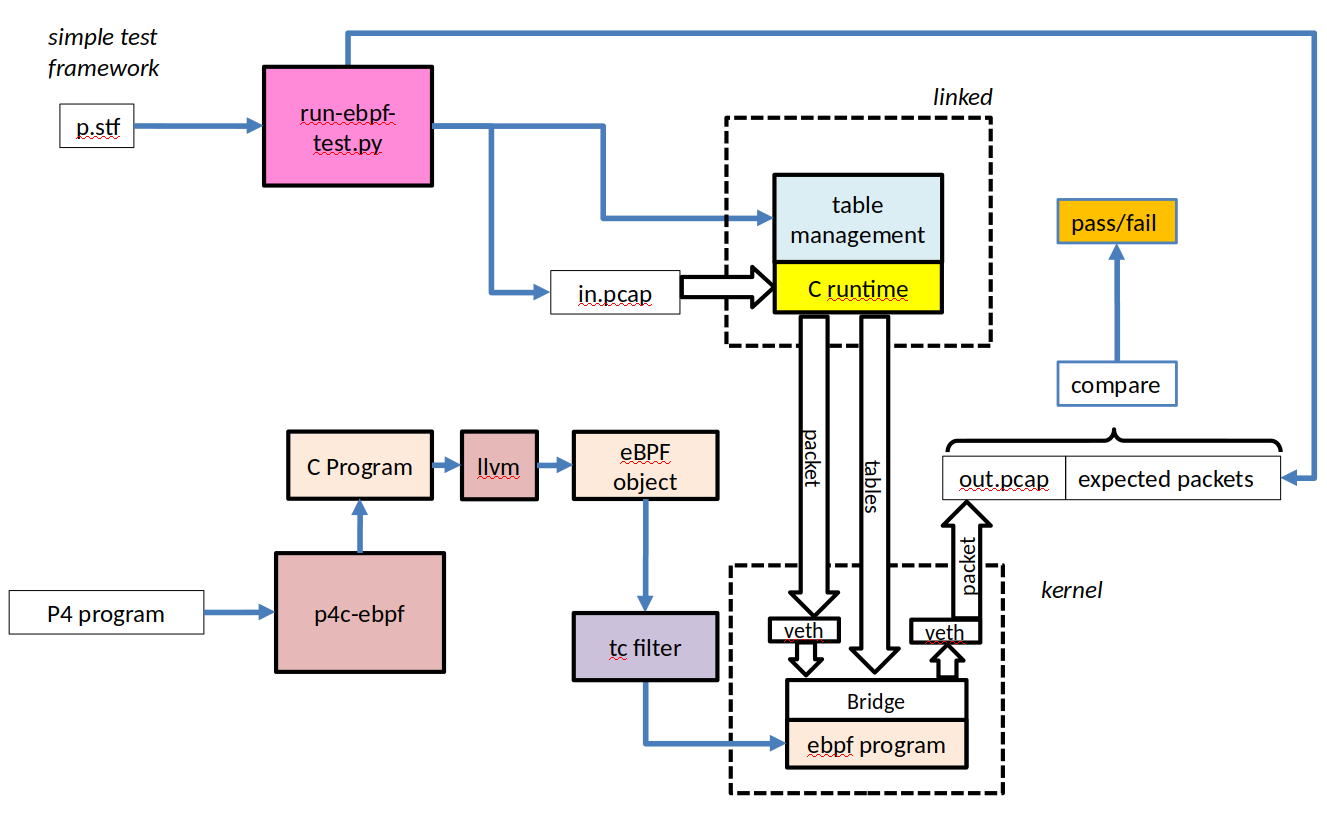
\includegraphics[width=0.7\linewidth]{kernel_test}
	\caption{}
	\label{fig:kernel_test}
\end{figure}